\chapter{Modeling Trajectory Planning as a MILP problem}
\label{section:modelingbasic}
\section{Introduction}
This section covers how a trajectory planning problem can be represented using Mixed Integer Linear Programming. This is a relatively simple model based on the work by Bellingham \cite{Bellingham2002}. This model by itself is sufficient to solve the trajectory planning problem, but its poor scalability prevents it from being used on any but the most basic scenarios. \\

Section \ref{subsec:milp-overview} starts out with a basic overview of what MILP is, highlighting its strengths and weaknesses. Section \ref{subsec:state} to \ref{subsec:obs-avoid} describe how I modeled the trajectory planning problem. 

%TODO: REWRITE
%MILP is a form of mathematical programming, form of declarative programming. contrast with imperative programming: say what the solution looks like instead of how to get there. Mathematical programming: subset of declarative programming where problem is defined as mathematical problem. Solver computes result.\\
%Big advantages: \\
%- dont need to say how it is done, focus is on precisely modeling problem.\\
%- flexible: can easily change rules: make problem more restrictive or relaxed, change the goal, etc ``just works''\\
%- can be really fast thanks to work on solvers\\
%\\
%disadvatages:\\
%- no free lunch (find reference): for anything more than very basic cases, solver cannot guarantee that a solution will be found any faster than random search\\
%	--> cant rely on just the solver doing the work, problem needs to be stated in a way that guides solver in the right direction
%	--> even when careful, as problem becomes more complex, solvers struggle\\
%-  hard to understand: solver finds solution or not.
%	-->Solution is optimal, but if it is not as expected it does not give any information why.
%	-->when no solution: can show which constraint failed, but problem is not necessarily there. complex interplay between constraints is extremely hard to debug\\





\section{Overview of MILP}
\label{subsec:milp-overview}
\subsection{Mathematical Programming}
Mixed integer linear programming is an extension of linear programming, which is in turn a form of mathematical programming. In mathematical programming, problems are represented as models. Each model has some amount of unknown decision variables. Models are solved by assigning values to those decision variables. \\
To accurately represent most problems, a model also needs constraints. Constraints are mathematical equations which determine the allowed values for each decision variable. When all decision variables have values which are allowed by the constraint, the constraint is called "satisfied". \\
In mathematical programming, solvers are used to assign values to variables in a model. The goal of a solver is to assign those values while ensuring that all constraints are satisfied. For many problems (and their corresponding models), this is extremely challenging. Only one solution may exist among a near infinite amount of options. \\
In many cases, the goal is not to find just any solution to the problem, but to find the best possible solution. The quality of a solution is determined by an objective function. The solver aims to find the solution with the highest (or lowest) score based on the objective function, while also keeping all constraints satisfied. When an objective function is present, these problems are called optimization problems. \\
\subsection{Mixed Integer Linear Programming}
There are many different subfields of mathematical programming. In these fields, the expressiveness of the model is usually traded against the the difficulty of solving a model. By limiting how a problem can be expressed in a model, it becomes much easier to build a solver which can efficiently solve those models. This is where Linear Programming (LP) comes in. In LP, all constraints must be linear equations. The objective function must also be a linear function. The decision variables must be real values. \\
Under those limitations, LP problems can be solved quickly and reliably \cite{Dantzig1963}. However, the kinds of problems that can be modeled using LP are very limited. It is impossible to model "OR" ($\vee$) relations, conditionals ( $\rightarrow$) and many other logical relations. It also prevents the use of common mathematical functions like the absolute value, among others. \\
Many of those limitations can be resolved by allowing some (or all) of the decision variables to be integers \cite{Mitra1994}. While variables could take on integer variables in LP, there is no way to limit the domain of a variable so it can only take on integer values. When at least one variable must take on an integer value, the technique is called Mixed-Integer Linear Programming (MILP). LP alone is not sufficient to model a trajectory planning problem, so MILP is required.\\
The addition of integer variables makes MILP much harder to solve than LP. MILP belongs to a class of problems called "NP-Complete". Problems which belong to this class tend to quickly become too difficult to solve in an acceptable amount of time when the size of the problem is increased. For MILP, the worst case difficulty grows exponentially with the amount of integer variables.
\subsection{Arguments for MILP}
The poor worst case performance is the main disadvantage of MILP, but it also has advantages over other approaches. \\
The main advantage is flexibility. Mathematical Programming is a form of declarative programming. In imperative programming, the programmer needs to describe step-by-step how the algorithm should solve a specific kind of problem. Even a small change to the problem may cause large changes to how the algorithm works.\\
In declarative programming, the programmer does not tell the computer exactly how to solve the problem. A general solver does the heavy lifting and finds the solution. This means that when the problem changes slightly, the model only needs to be updated to reflect that small change. \\
Performance could actually be an advantage. Planning a good trajectory is not a trivial problem, so performance is likely to be a concern for any competing algorithm. MILP solvers have been used in other industries for decades, so a lot of work has gone in to making those solvers fast and memory-efficient. The performance of MILP approach could be comparable to, or even exceed, the performance of other algorithms.

%there is a single (linear) target function which needs to be minimized or maximized by the solver. For the work in this paper, we used the IBM CPLEX solver. A problem typically also contains a number linear inequalities which constrain the values of the variables in the target function. \\
%\begin{figure}
%\begin{math}
%\text{maximize} \quad f(\boldsymbol{x}) = a_0 x_0 + a_1 x_1 + ...\\
%\text{subject to} \\
%b_{0,0} x_0 + b_{0,1} x_1 + ...\leq c_0 \\
%b_{1,0} x_0 + b_{1,1} x_1 + ...\leq c_1 \\
%... \\
%x_0, x_1, ... \in \mathbb{R}
%\end{math}
%\caption{A typical linear problem}
%\label{fig:example-lp}
%\end{figure}
%In the example in figure \ref{fig:example-lp}, $  f(\boldsymbol{x}) $ is the linear goal function to be maximized. When a symbol is in \textbf{bold}, it represents a vector, otherwise it represents a scalar value. In this case, $\boldsymbol{x}$ is the vector containing all variables $x_i$. The linear inequalities below the goal function are the constraints as linear inequalities with coefficients $b_{j,i}$ and the maximum value $c_j$. The final line ensures that all variables have a real domain. When some (or all) of the variables have an integer domain, the problem is a mixed integer problem. \\
%Using multiple inequalities and possibly additional variables, it is possible to model more complex mathematical relations. Some of those relations, like logical operators or the absolute value function, can only be expressed when integer variables are allowed \cite{Mitra1994}. 
\section{Time and UAV state}
\label{subsec:state}

The trajectory planning problem can be represented using discrete time steps. The state of the UAV (position, velocity, etc.) is defined at each time step. Time steps are spaced out regularly, with $\Delta t$ between them. The progression of time is modeled by Equation \ref{eq:t-start} and \ref{eq:t-rest}. $time_n$ represents the amount of time that has passed at a given time step $n$. Equation \ref{eq:t-start} initializes the time at the first time step to be zero. Equation \ref{eq:t-rest} progresses time by $\Delta t$ at each time step. In total, there are $N$ time steps.

\begin{equation}
\label{eq:t-start}
time_0 = 0
\end{equation}
\begin{equation}
\label{eq:t-rest}
time_{n+1} = time_{n} + \Delta t,  \quad 0 \leq n < N - 1
\end{equation}

The position of the UAV at time step $n$ is represented by $p_n$. Equation \ref{eq:p-start} initializes the position in the first time step to the starting position $\boldsymbol{p}_{start}$. Equation \ref{eq:p-rest} updates the position of the UAV in the next time step, based on the velocity $\boldsymbol{v}_n$ in the current time step and time step size $\Delta t$. When a variable is in \textbf{bold}, it represents a vector instead of a scalar value.

\begin{equation}
\label{eq:p-start}
\boldsymbol{p}_0 = \boldsymbol{p}_{start}
\end{equation}
\begin{equation}
\label{eq:p-rest}
\boldsymbol{p}_{n+1} = \boldsymbol{p}_{n} + \Delta t * \boldsymbol{v}_{n}  \quad 0 \leq n < N - 1
\end{equation}

The velocity of the UAV is modeled the same way as the position. Equation \ref{eq:v-start} initialized the velocity in the first time step, and Equation \ref{eq:v-rest} updates it at each time step based on the acceleration $\boldsymbol{a}_i$. Other derivatives can be modeled like this as well.

\begin{equation}
\label{eq:v-start}
\boldsymbol{v}_0 =\boldsymbol{v}_{start}
\end{equation}
\begin{equation}
\label{eq:v-rest}
\boldsymbol{v}_{n+1} =\boldsymbol{v}_{n} + \Delta t * \boldsymbol{a}_{n}  \quad 0 \leq n < N - 1
\end{equation}

\section{Objective function}
\label{subsec:obj-fun}
The objective for the solver is to minimize the amount of time steps before the UAV reaches the goal position. Equation \ref{eq:goal-fun} describes this. $done_n$ is a boolean variable which is $true$ when the UAV has reached the goal on or before time step $n$. A boolean variable is an integer variable which can only be $0$ (false) or $1$ (true).


\begin{equation}
\label{eq:goal-fun}
minimize \quad - \mathlarger{\sum}_{n=0}^{n < N} done_n
\end{equation}

The value of $done_{n+1}$ at time step $n + 1$ is true if either $done_n$ is true, or a state transition $cdone_{n+1}$ occurs. The state transition flag $cdone_{n+1}$ is true whenever all conditions for reaching the goal have been satisfied. This is expressed in Equation \ref{eq:fin-rest}.

\begin{equation}
\label{eq:fin-rest}
done_{n+1} = done_n \vee cdone_{n+1},  \quad 0 \leq n < N  - 1
\end{equation}

This formulation is nearly correct, but fails to address two important assumptions. The first assumption is that the UAV has not reached its goal at the start of the trajectory. $done_0$ is not constrained by Equation \ref{eq:fin-rest}, so a valid (and optimal) solution would be setting $done_0$ to $true$. Equation \ref{eq:fin-start} resolves this issue by forcing $done_0$ to be false.

\begin{equation}
\label{eq:fin-start}
done_0 = 0
\end{equation}

Similarly, no constraints actually force the UAV to reach its goal. The value of the objective function would be poor, but the solution would be valid. Equation \ref{eq:fin-end} forces $done_{N-1}$ to be true at the last time step. In combination with Equation \ref{eq:fin-rest} and \ref{eq:fin-start}, this ensures that the UAV must reach its goal eventually for the solution to be valid.

\begin{equation}
\label{eq:fin-end}
done_{N - 1} = 1
\end{equation}

To model the state transition, represented by $cdone_{n}$, Lamport's \cite{Lamport1989} state transition axiom method was used. This method separates the value of the state ($done_{n}$) from the requirements for transition ($cdone_{n}$). Equation \ref{eq:fin-rest} is the first part: it expresses that the state changes when a transition event occurs. It is not concerned with what leads to that state transition. \\
The second part is Equation \ref{eq:cfin}: It describes the requirements for a state transition to occur. In this case, the UAV must be at its goal position (represented by $cdone_{p,n}$) and not be done already at time step $n$.

\begin{equation}
\label{eq:cfin}
cdone_n =  cdone_{p,n} \wedge \neg done_n\quad 0 \leq n < N
\end{equation}

The equations discussed so far are all in a general form which apply to a UAV moving through a world with an arbitrary amount of spatial dimensions. For this thesis, the assumption is that the UAV moves through a 2D world. Starting from Equation \ref{eq:cfin-p}, some equations only apply to 2D worlds for simplicity. \\
Equation \ref{eq:cfin-p} defines when the UAV is considered to be at the goal position. $x_n$ and $y_n$ are the UAV's 2D coordinates at time step $n$, while $x_{goal}$ and $y_{goal}$ are the coordinates of the goal position. The UAV has reached the goal if each coordinate is at most $\epsilon{p}$ away from the goal's matching coordinate
\begin{equation}
\label{eq:cfin-p}
cdone_{p,n} = |x_{n} - x_{goal}| < \epsilon_{p} \wedge  |y_{n} - y_{goal}| < \epsilon_{p}, \quad 0 \leq n < N
%cfin_{p,n} =  \mathlarger{\mathlarger{\bigwedge_{i = 0}^{i < Dim(\boldsymbol{p}_n)}}} |p_{n,i} - p_{goal, i}| < \epsilon_{p},  \quad 0 \leq n \leq N
\end{equation}

Adding additional requirements for the state transition is easy. As an example, we may wish to ensure that the UAV stops at its goal. Equation \ref{eq:cfin} can be extended with a $cdone_{v,n}$ requirement as shown in \ref{eq:cfin-2}. $cdone_{v,n}$ is defined by Equation \ref{eq:cfin-v}, where $vx_n$ and $vy_n$ are the components of the UAV's velocity vector which must be smaller than some $\epsilon_v$.

\begin{equation}
\label{eq:cfin-2}
cdone_n =  cdone_{p,n} \wedge cdone_{v,n} \wedge \neg done_n\quad 0 \leq n < N
\end{equation}

\begin{equation}
\label{eq:cfin-v}
cdone_{v,n} = |vx_{n}| < \epsilon_{v} \wedge  |vy_{n}| < \epsilon_{v}, \quad 0 \leq n < N
\end{equation}
\section{UAV state limits}
\label{subsec:state-limits}
\begin{figure}
    \centering
        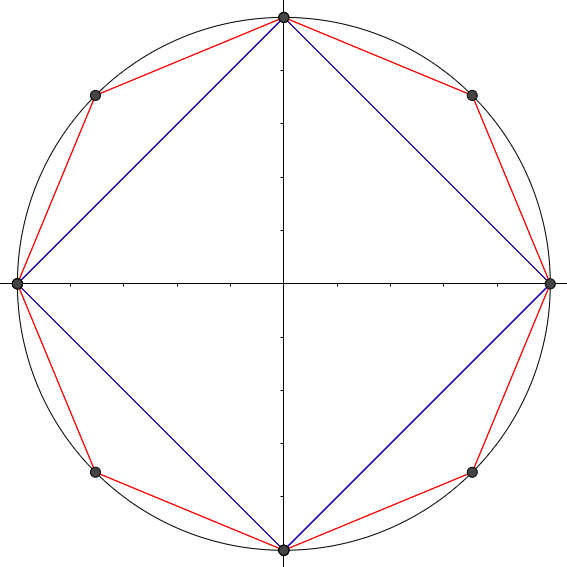
\includegraphics[width=0.4\columnwidth]{img/circlelinear}
    \caption[A visualization of the linear approximation for the 2-norm]{If the velocity is limited to a finite value, the velocity vector must lie within the circle centered on the origin with the radius equal to that value. This is represented by the black circle. This circle cannot be approximated in MILP, but it can be approximated using several linear constraints. The blue square shows the approximation using 4 linear constraints. The red polygon uses 8 linear constraints. As more constraints are used, the approximation gets closer and closer to the circle. }\label{fig:circlelinear}
\end{figure}
Like any vehicle, a UAV has a certain maximum velocity. The model should contain constraints which prevent the UAV from moving faster than the maximum velocity. The magnitude of the velocity is the 2-norm of the velocity vector (which is Pythagoras' theorem for a 2D vector). This cannot be represented as a linear constraint because the components of the velocity vector need to be squared. However, the 2-norm can be approximated using multiple linear constraints. 
\par
Figure \ref{fig:circlelinear} visualizes how this works for the 2D case. All velocity vectors with a magnitude smaller than the maximum velocity are on the inside of the black circle with radius $v_{max}$. This cannot be expressed in MILP, but a regular polygon which fits inside the circle can be expressed. As the amount of vertices $N_{vertex}$ making up the polygon increases, the approximation gets more and more accurate. The coordinates of the vertices of the polygon, $q_{x,i}$ and $q_{y,i}$ are defined by Equations \ref{eq:maxvel-theta}-\ref{eq:maxvel-points-y} in counter-clockwise order.

\begin{figure}[!t]
    \centering
    
    \begin{subfigure}[t]{0.3\textwidth}
        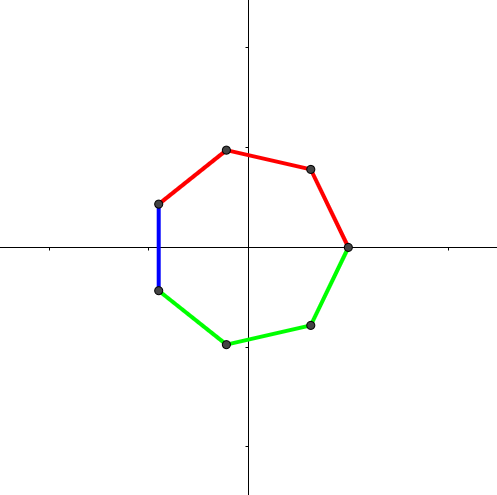
\includegraphics[width=\textwidth]{linear-part-1}
        \caption{}
        \label{fig:linear-part-1}
    \end{subfigure}
    \hfil
    \begin{subfigure}[t]{0.3\textwidth}
        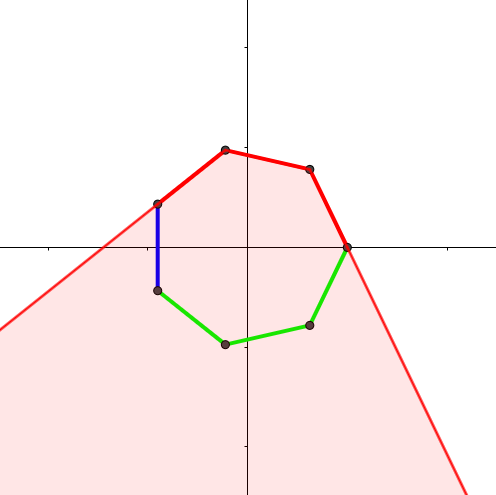
\includegraphics[width=\textwidth]{linear-part-2}
        \caption{}
        \label{fig:linear-part-2}
    \end{subfigure}
    \hfil    
    \begin{subfigure}[t]{0.3\textwidth}
        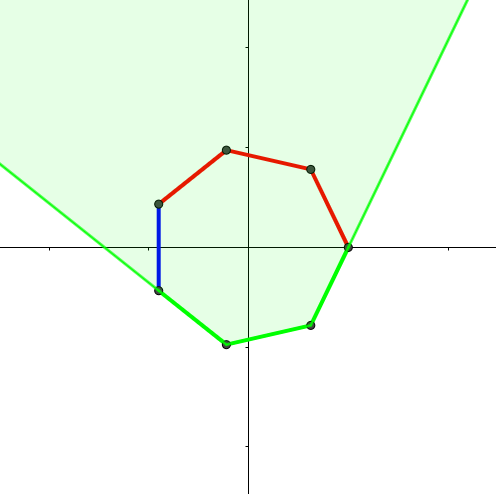
\includegraphics[width=\textwidth]{linear-part-3}
        \caption{}
        \label{fig:linear-part-3}
    \end{subfigure}
    \hfil    
    \begin{subfigure}[t]{0.3\textwidth}
        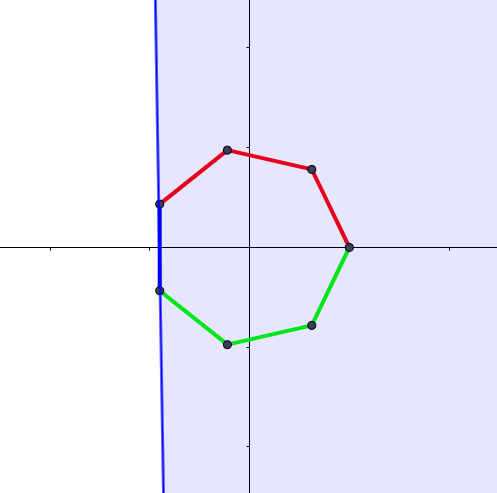
\includegraphics[width=\textwidth]{linear-part-4}
        \caption{}
        \label{fig:linear-part-4}
    \end{subfigure}
    \hfil    
    \begin{subfigure}[t]{0.3\textwidth}
        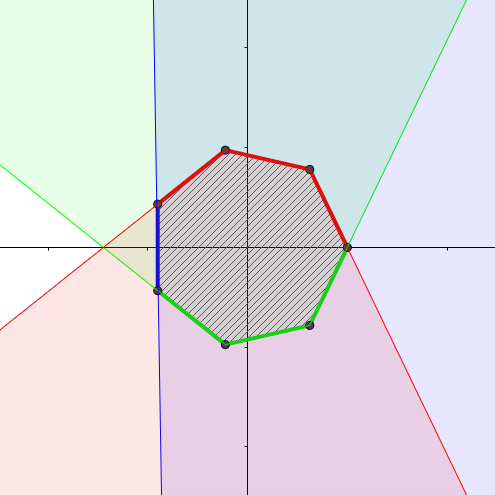
\includegraphics[width=\textwidth]{linear-part-5}
        \caption{}
        \label{fig:linear-part-5}
    \end{subfigure}
    \caption[A visual demonstration of how the maximum velocity is constrained]{A visual demonstration of the equations that limit the maximum velocity. \ref{fig:linear-part-1} shows how the polygon is divided into the top part, bottom part, and the left edge. \ref{fig:linear-part-2} shows the region allowed by the edges on the top part of the polygon in red. This region is determined by Equation \ref{eq:vmax-1}. \ref{fig:linear-part-3} shows the same in green for the bottom part, as determined by \ref{eq:vmax-2}. Finally  \ref{fig:linear-part-4} shows the region allowed by the left edge in blue, as determined by Equation \ref{eq:vmax-3}. The velocity vector must remain in all three regions. As seen in \ref{fig:linear-part-5}, the shape where all three regions overlap is exactly the initial polygon. }\label{fig:linear-demo}
\end{figure}



\begin{equation}
\label{eq:maxvel-theta}
\theta = \dfrac{2\pi}{N_{points}}
\end{equation}
\begin{equation}
\label{eq:maxvel-points-x}
q_{x,i}  = v_{max} * cos( \theta i), \quad 0 \leq i < N_{points}
\end{equation}
\begin{equation}
\label{eq:maxvel-points-y}
q_{y,i}  = v_{max} * sin( \theta i), \quad 0 \leq i < N_{points}
\end{equation}
Like before, the equations are limited to the 2D case, but can be extended to 3D as well. Each edge of the polygon defines a line with slope $a_i$ and intercept $b_i$, as determined by Equations \ref{eq:lin-delta}-\ref{eq:lin-b}.

\begin{equation}
\label{eq:lin-delta}
\Delta q_{x,i} = q_{x,i} - q_{x,i-1}, \quad \Delta q_{y,i} = q_{y,i} - q_{y,i-1}
\end{equation}
\begin{equation}
\label{eq:lin-a}
a_i = \dfrac{\Delta q_{y,i}}{\Delta q_{x,i}} \quad 0 \leq i < N_{vertex}
\end{equation}
\begin{equation}
\label{eq:lin-b}
b_i = q_{y,i} - a_i q_{x,i}  \quad 0 \leq i < N_{vertex}
\end{equation}




Finally, the constraints can be constructed using the slope and intercepts of each line segment. For the edges on the "top" half of the polygon, the velocity vector must stay \emph{below} those edges. This is expressed by Equation \ref{eq:vmax-1}. Similarly, for the bottom half, the velocity vector must stay \emph{above} those edges as expressed by Equation \ref{eq:vmax-2}. If $N_{vertex}$ is odd, the left-most edge of the polygon is vertical. Equation \ref{eq:vmax-3} handles this special case: the velocity vector must stay on the right of the left-most edge. This is illustrated by Figure \ref{fig:linear-demo}.



\begin{align}
vy_{n} &\leq a_i vx_{n} + b_i,  & \Delta q_{x,i} < 0, \quad 0 \leq n < N  \label{eq:vmax-1} \\
vy_{n} &\geq a_i vx_{n} + b_i,  & \Delta q_{x,i} > 0, \quad 0 \leq n < N \label{eq:vmax-2} \\
vx_{n} &\geq q_{x,i},  & \Delta q_{x,i} = 0, \quad 0 \leq n < N \label{eq:vmax-3}
\end{align}

The acceleration and other vector properties of the vehicle can be limited in the same way. 

\section{Obstacle avoidance}
\label{subsec:obs-avoid}

The last element of the model is obstacle avoidance. Obstacles are regions in the world where the UAV is not allowed to be. This may be due to a physical obstacle, but it could also be a no-fly zone determined by law or other concerns. \\
Assuming that each obstacle is a 2D convex polygon, the constraints for obstacle avoidance are similar to those of the vehicle state limits in Section \ref{subsec:state-limits}. However, the big difference is that the UAV must stay on the outside of the polygon instead of the inside. \\

\begin{figure}[h]
    \centering
    
    \begin{subfigure}[]{0.25\textwidth}
        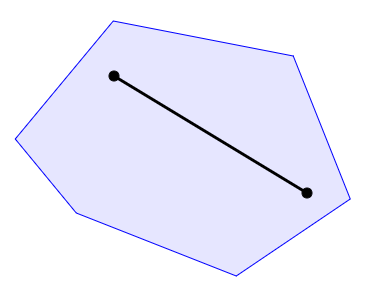
\includegraphics[width=\textwidth]{convex}
        \caption{A convex shape}
        \label{fig:convex-example}
    \end{subfigure}
    \hfil
    \begin{subfigure}[]{0.25\textwidth}
        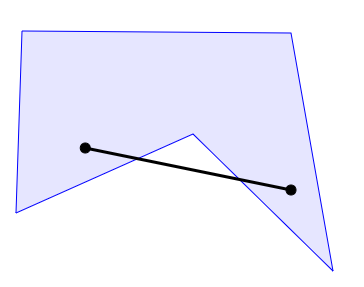
\includegraphics[width=\textwidth]{nonconvex}
        \caption{A non-convex shape}
        \label{fig:nonconvex-example}
    \end{subfigure}
    \caption[A demonstration of the difference between a convex and nonconvex shape]{A demonstration of the difference between convex and nonconvex shapes. In a convex shape, the line between any two points inside the shape must be fully contained inside that shape. If this is not the case, the shape is nonconvex.}\label{fig:convexity-example}
\end{figure}

\subsection{Importance of Convexity}
The maximum velocity is modeled without using any integer variables. This is possible because the allowed region for the velocity vector is a convex shape. A shape is convex if a line drawn between any two points inside that shape is also fully inside the shape. This is demonstrated in Figure \ref{fig:convex-example}\\
This property does not hold for obstacle avoidance. If the UAV is on one side of an obstacle, it cannot move in a straight line to the other side of that obstacle. Because of that obstacle, the shape formed by all the positions where the UAV is allowed to be is no longer convex. This can be seen in Figure \ref{fig:nonconvex-example}. \\
To express non-convex constraints, integer variables are needed. This causes the difference between what can be modeled in Linear Programming versus Mixed-Integer Linear Programming: non-convex constraints can be expressed in MILP, while this is not possible in LP.



\begin{figure}[!t]
    \centering
    
    \begin{subfigure}[t]{0.47\textwidth}
        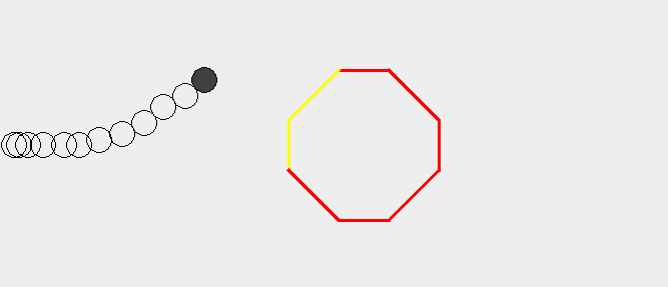
\includegraphics[width=\textwidth]{img/obs1}
        \caption{}
    \end{subfigure}
    \hfil
    \begin{subfigure}[t]{0.47\textwidth}
        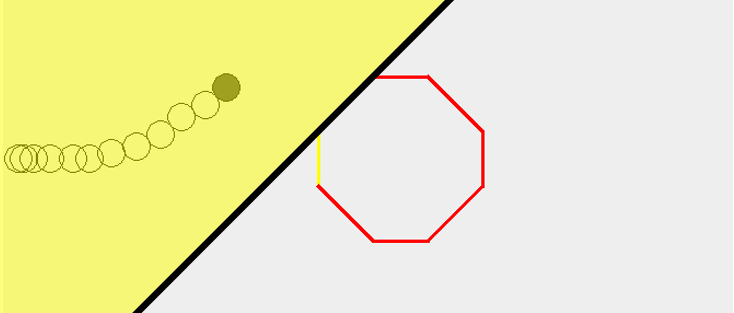
\includegraphics[width=\textwidth]{img/obs2}
        \caption{}
    \end{subfigure}
    \par\bigskip
    \begin{subfigure}[t]{0.47\textwidth}
        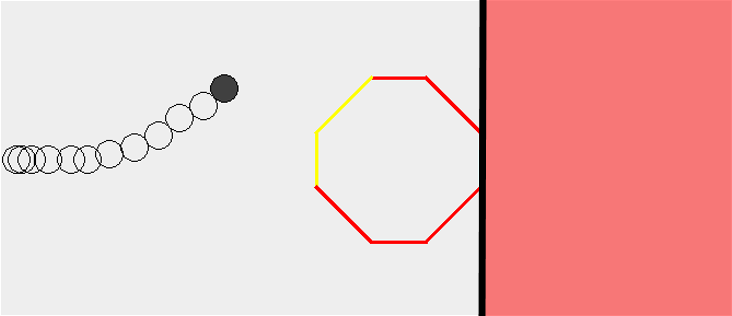
\includegraphics[width=\textwidth]{img/obs3}
        \caption{}
    \end{subfigure}
    \caption[A visual demonstration of obstacle avoidance in the MILP model]{A visual representation of how obstacle avoidance works. The top image shows the UAV's current position as the filled circle, with its path in previous time steps as hollow circles. The color of the edges of the obstacle represent whether or not the UAV is in the safe zone for that edge. An edge is yellow if the UAV is in the safe zone, and red otherwise. The middle image shows the safe zone defined by a yellow edge in yellow. Note how the UAV is on one side of the black line and the obstacle is entirely on the other side. The UAV cannot collide with the obstacle as long as it is on the opposite side of the line as the obstacle. The bottom image shows an edge for which the UAV is not in the safe zone (represented in red this time). The vehicle is on the same side of the line as the obstacle, so a collision cannot be ruled out. As long as the vehicle is in the safe zone of at least one edge, it cannot collide with the obstacle.}\label{fig:obs}
\end{figure}

\subsection{Big M Method}
Like with the maximum velocity in Section \ref{subsec:state-limits}, the edges of the obstacle are used to construct the constraints. Each edge defines a line, as determined by Equations \ref{eq:lin-delta}-\ref{eq:lin-b}. If the obstacle is convex, the obstacle will be entirely on one side of that line. If the UAV is on the other side, the one without the obstacle, it cannot collide with that obstacle. This region can be consider the safe region defined by that edge. As long as the UAV is in the safe region of at least one edge, no collisions can occur. Figure \ref{fig:obs} demonstrates this visually. \\
A popular way to model this is the "Big M" method \cite{Schouwenaars2001}. For each edge, a constraint is constructed which forces the UAV to be in the safe region for that edge. However, the UAV must only be in the safe region of at least one edge. This means that it must be possible to "turn off" constraints. \\
For each edge of an obstacle, a boolean $slack$ variable is used to represent whether the constraint for that edge is enabled. If this $slack$ variable is $true$ (equal to $1$), the constraint is \emph{disabled}. This is where the "Big M" comes in: the $slack$ variable is multiplied by a very large number $M$ on one side of the inequality constraint for that edge. $M$ must be chosen to be large enough to ensure that ,when $slack$ is $true$, the inequality is always satisfied. \\
In Equations \ref{eq:obs-m-1}-\ref{eq:obs-m-4} below, $q_{x,i}$ and $q_{y,i}$ are the 2D coordinates of vertex $i$ of the obstacle. The slope $a_{i}$ and intercept $b_{i}$ of edge $i$ are calculated as in Equations \ref{eq:lin-delta}-\ref{eq:lin-b}. For every time step $n$:
\\
\begin{align}
y_{n} \quad + \quad M*slack_{i,n} \quad &\geq 
\quad a_{i} x_{n} + b_{i},  	
& \Delta q_{x,i} < 0 							 	
\label{eq:obs-m-1} \\
y_{n} \quad - \quad M*slack_{i,n} \quad &\leq 
\quad a_{i} x_{n} + b_{i},
& \Delta q_{x,i} > 0 							 	
\label{eq:obs-m-2} \\
x_{n} \quad - \quad M*slack_{i,n} \quad &\leq
\quad  q_{x,i}, 		
& \Delta q_{y,i} < 0, \quad \Delta q_{x,i} = 0 	
\label{eq:obs-m-3} \\
x_{n} \quad + \quad M*slack_{i,n} \quad &\geq 
\quad q_{y,i},  		
& \Delta q_{y,i} > 0, \quad \Delta q_{x,i} = 0 	
\label{eq:obs-m-4}
\end{align}
\\
Like in Equations \ref{eq:vmax-1} and \ref{eq:vmax-2}, edges on the top and bottom of the obstacle are treated differently. Equation \ref{eq:obs-m-1} covers the top edges. The UAV must be above the edge. If the UAV is not above the edge (when $y_n$ is too small), enabling $slack_{i,n}$ will add $M$ on the left-hand side of the inequality and ensure that it is always larger than the right-hand side. Equation \ref{eq:obs-m-2} does the same for edges on the bottom. The inequality is flipped around so that the UAV must be below the edge. This also means that $M$ must be subtracted from the left-hand side of the inequality to ensure the constraint is always satisfied. \\
Vertical edges are also possible. A vertical edge may occur on the left or right side of the polygon, similar to what Figure \ref{fig:linear-part-4} shows for the left side. These are covered by Equations \ref{eq:obs-m-3} and \ref{eq:obs-m-4} respectively.\\
Finally Equation \ref{eq:obs-slack} ensures that at least one of the slack variables must be false at each time step.
\\
\begin{equation}
\neg \mathlarger{\mathlarger{\bigwedge_{i}}} slack_{i,n} \quad 0 \leq n \leq N
\label{eq:obs-slack}
\end{equation}
\\
Equations \ref{eq:obs-m-1} - \ref{eq:obs-m-4} assume that the UAV has no physical size. The position of the UAV is the position of its center of mass. Because a UAV has certain physical dimensions, it will collide with an obstacle before its center of mass reaches the obstacle. The vehicle's shape is approximated as a circle with radius $r$. The vertical offset $o_i$ required to move the line with slope $a_i$ from the center of the circle to the edge is calculated by Equation \ref{eq:offset}. A geometric proof is given in Figure \ref{fig:offset-proof} on page \pageref{fig:offset-proof}.
\\
\begin{equation}
o_{i} = r \sqrt{1 + a_i^2}
\label{eq:offset}
\end{equation}
\\
With the vertical offset calculated, Equations \ref{eq:obs-m-1} - \ref{eq:obs-m-4} can be extended to Equations \ref{eq:obs-m-1-v}-\ref{eq:obs-m-2-v} which take the UAV size into account.
\\
\begin{align}
y_{n} + M*slack_{i,n} \quad &- \quad o_i \quad \geq 
\quad a_{i} x_{n} + b_{i},  	
& \Delta q_{x,i} < 0 							 	
\label{eq:obs-m-1-v} \\
y_{n} - M*slack_{i,n} \quad &+ \quad o_i \quad \leq 
\quad a_{i} x_{n} + b_{i},
& \Delta q_{x,i} > 0 							 	
\label{eq:obs-m-2-v} \\
x_{n} - M*slack_{i,n} \quad &+ \quad r \quad \leq
\quad  q_{x,i}, 		
& \Delta q_{y,i} < 0, \quad \Delta q_{x,i} = 0 	
\label{eq:obs-m-3-v} \\
x_{n} + M*slack_{i,n} \quad &- \quad r \quad \geq 
\quad q_{y,i},  		
& \Delta q_{y,i} > 0, \quad \Delta q_{x,i} = 0 	
\label{eq:obs-m-4-v}
\end{align}

\begin{figure}
    \centering
        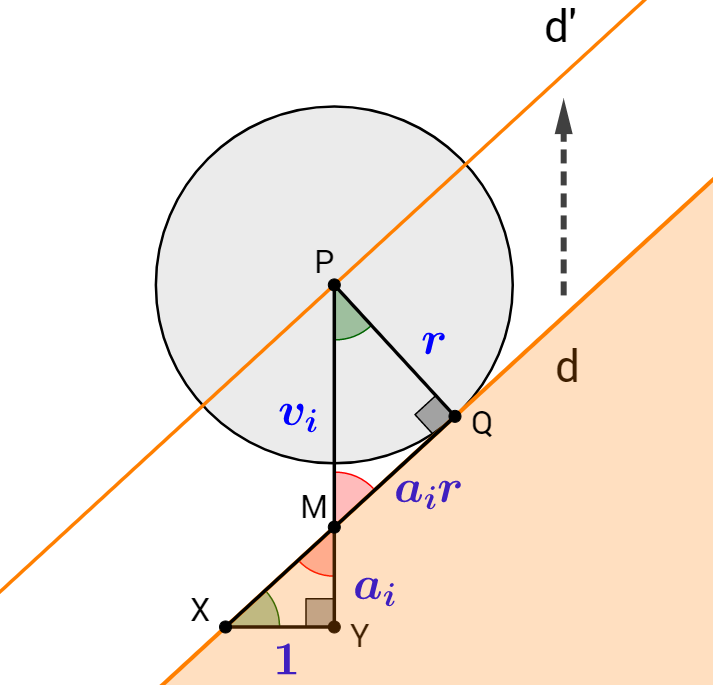
\includegraphics[width=0.8\columnwidth]{offset}
    \caption[A geometric proof for Equation \ref{eq:offset}]{A geometric proof for the vehicle offset formula in Equation \ref{eq:offset}. Measures are marked in blue. $P$ is the center of mass of the UAV. $d$ is the line defined by edge $i$ of an obstacle. The obstacle is the orange region. We wish to translate $d$ vertically to $d'$ such that when the UAV's center of mass $P$ touches $d'$, the circle with radius $r$ (representing the UAV's shape, colored in grey) touches $d$ in $Q$. If $d'$ is used for the constraint instead of $d$, the UAV cannot collide with the obstacle. The difference between the intercepts of $d$ and $d'$ is $o_i = |PM|$. The slope of $d'$ is $a_i$, so if $XY$ is horizontal and $|XY| = 1$, then $|MY| = a_i$. Corner $M$ is the same in both triangle $PQM$ and $XYM$, as marked in red. Corner $Q$ and $Y$ are both right angles. This means $PQM$ and $XYM$ are similar triangles. As a result: if $|PQ| = r$, then $|QM| = a_ir$. Using Pythagoras' theorem: $o_i = \sqrt{r^2 + a_i^2r^2} = r\sqrt{1+a_i^2}$.}\label{fig:offset-proof}
\end{figure}